%\documentclass[pre,floatfix,onecolumn, 12pt]{revtex4-1} 
\documentclass[12pt,a4paper]{article}
\usepackage[utf8]{inputenc}
\usepackage[spanish]{babel}
\usepackage{amsmath}
\usepackage{amsfonts}
\usepackage{amssymb}
\usepackage{graphicx}
\usepackage{lmodern}
\usepackage{authblk}
\usepackage[hyphens,spaces,obeyspaces]{url}
\usepackage[colorlinks,allcolors=blue]{hyperref}
\usepackage{verbatim}

\begin{document}

\author{K. F. Laneri$^1$ y A. B. Kolton$^{1,2}$}
\affil{$^1$ CNEA, CONICET, Centro At\'omico Bariloche, (8400) Bariloche, Argentina}
\affil{$^2$ Instituto Balseiro (UNCu)}

\title{Diagramas de Riesgo: {\it Significado, Implementación y Uso}}

\maketitle

\abstract{
En este documento se describe un índice de riesgo epidemiológico basado 
en la serie temporal de casos positivos diarios de COVID19 en una población dada. 
El índice de riesgo estima la cantidad de casos positivos esperables 
en los próximos días y puede usarse para estimar el número de cuidados intensivos adicionales que se necesitarán 
en los hospitales o el número de personas que requerirán de 
un seguimiento.
}
%\tableofcontents



\begin{figure}
%\begin{center}
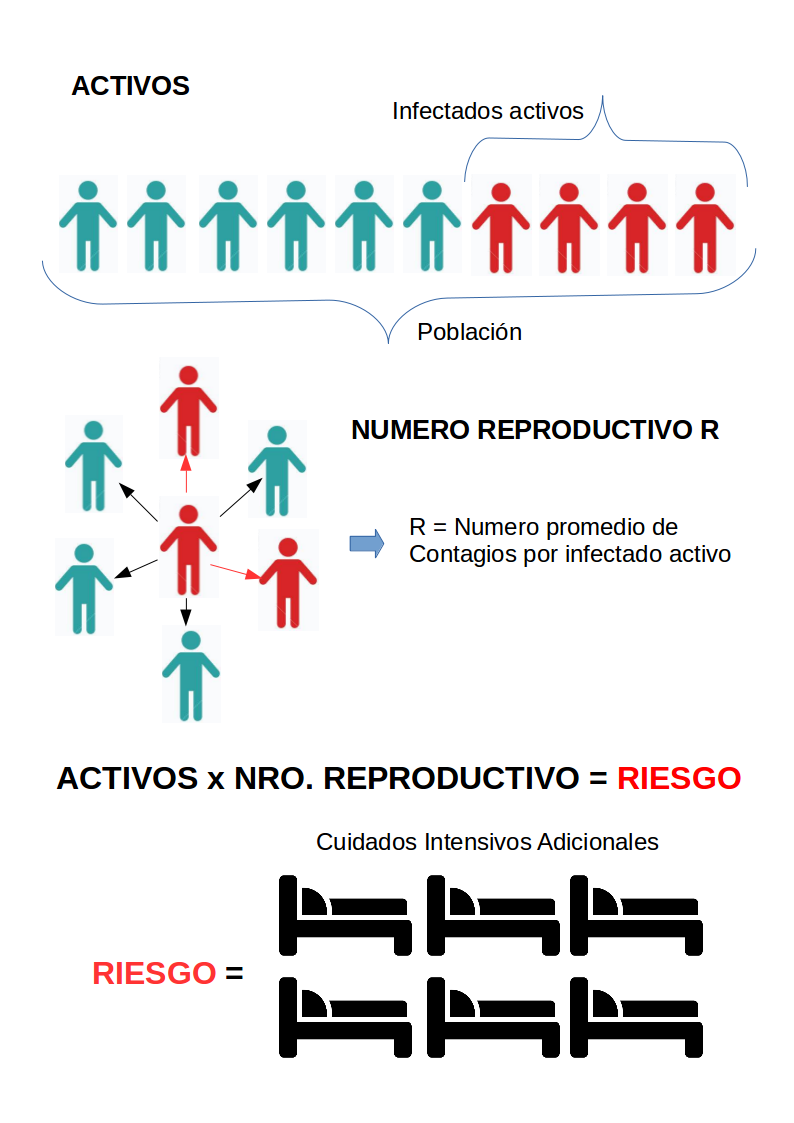
\includegraphics[width=14cm,clip=true]{explicacion.png}
%\end{center}
\caption{
Explicación gráfica del uso del número de reproducción 
empírico y el número de casos activos para 
la predicción de un índice de riesgo sanitario.
}
\label{fig:riesgo}
\end{figure}

\section*{Número Reproductivo Empírico}
En epidemiología matemática clásica se utiliza el Número Reproductivo Efectivo 
{\cal R} para medir la velocidad con la que se propaga una epidemia a un tiempo dado. 
Es una medida del número medio de personas infectadas por una persona 
infecciosa durante su período activo. Es decir, el número de casos secundarios por cada caso primario. 
A menudo se habla del número reproductivo básico $R_0$, que es el valor 
de $R_t$ a tiempo cero ($t=0$), es decir, antes de que se inicie 
la propagación de la epidemia, sin intervención alguna, en una 
población susceptible en equilibrio. El número de reproducción empírico 
en cambio monitorea la velocidad de contagio en función del tiempo durante la epidemia, 
es susceptible a las intervenciones y a los distintos eventos que producen 
brotes epidémicos.


Para evaluar el Número Reproductivo Empírico, primero definimos $R_t$, que
se estima a partir del número de casos positivos diarios reportados $N_t$, 
donde $t$ es el número de día que corresponde al inicio de síntomas del caso 
positivo. Para eliminar fluctuaciones en $N_t$, usamos una 
ventana de casos de tres días y la dividimos por la misma ventana corrida $5$ 
días atrás:
\begin{equation}
R_t = \frac{N_{t-1}+N_{t}+N_{t+1}}{N_{t-6}+N_{t-5}+N_{t-4}}
\end{equation}
El desplazamiento de $\sim 5$ días contempla, 
de forma empírica, el hecho de que una persona recién 
infectada (tenga o no síntomas) no infecta inmediatamente a otras personas, 
sino luego de un cierto número de días característico de la enfermedad.
Es decir, la dinámica de contagio contiene tiempos de espera o demoras. 
El número $R_t$ mide entonces 
la tasa de multiplicación de casos. Como sólo nos basamos 
en el número de casos positivos reportados, $R_t$ es una medida 
cuantitativa para estimar cuántas personas en promedio arrojarán un 
resultado positivo en sus testeos de mañana por cada 
persona testeada positiva hoy. Si suponemos que el número total 
de personas infectadas (incluyendo asintómaticos y sintómaticos no testeados) 
es proporcional al número de casos positivos reportados, entonces el número estimado
$R_t$ vale para todo el conjunto de casos, aún los no testeados.



En la práctica, $R_t$ tiene fuertes fluctuaciones, especialmente en poblaciones 
no muy grandes o en poblaciones con una dinámica de contagio muy heterogénea. 
Las fluctuaciones pueden tener su origen en un gran número de factores, 
desde retraso en la carga de los datos o la falta de carga de la 
fecha de inicio de síntomas, hasta la ocurrencia de eventos sociales de distinta índole. 
Dichas fluctuaciones complican la evaluación de tendencias, y afectan la calidad de la 
predicción. Para minimizarlas realizamos a su vez 
un promedio del valor de $R_t$ en una ventana de 7 días, 
definiendo el Número $R^7_t$ :

\begin{equation}
R^7_t = \sum_{i=-3}^{3} \frac{R_{t+i}}{7} = 
\frac{R_{t-3}+R_{t-2}+R_{t-1}+R_t+R_{t+1}+R_{t+2}+R_{t+3}}{7}
\end{equation}

\subsection*{Efectos de Borde}
La definición de $R^7_t$ tiene claramente 
un problema cuando $t$ se acerca al presente, porque 
puede ocurrir que $R_{t+3}$, $R_{t+2}$, o $R_{t+1}$ no puedan 
ser calculados, ya que necesitaríamos el reporte de casos 
futuros. Para minimizar este problema recurrimos a la estrategia 
de completar $N_t$, solo cuando sea necesario, 
usando extrapolación hacia adelante. Para ello 
calculamos el promedio de $N_t$ en una ventana de 7 días 
y usamos ese valor para completar la serie $N_t$ los 
días necesarios. 
Esta extrapolación solamente es necesaria hacerla 
cuando el tiempo considerado es tal que $t>hoy-4$ días. Dicha corrección minimiza los efectos de borde 
pero no evita completamente que los valores 
$R^7_t$ para los tiempos más recientes 
sufran un ligero reajuste en los próximos días 
hasta estabilizarse en un valor definido 
cuando $t<hoy-4$ días.  

\section*{Número De Casos Activos}

Si conocemos $R^7_i$ tenemos un índice que nos mide el número de personas 
que se infectan por cada persona infecciosa. Este número,
multiplicado por el número de personas infecciosas hoy, nos da la 
cantidad de personas que se infectarán mañana.
Pero no sabemos exactamente el número de personas infecciosas de hoy. 
Lo que sabemos es que el número de personas infecciosas hoy es aproximadamente 
proporcional al número de casos positivos de los últimos 14 días, 
porque $14$ días es aproximadamente el tiempo de recuperación de un infectado.

La incidencia acumulada en los últimos 14 días $A^{14}_t$ mide el número de personas cuyo testeo dió positivo en los últimos 14 días por cada 100~mil habitantes (la elección de 100~mil es arbitraria pero fija una escala de valores muy conveniente para la visualización y la comparación de poblaciones). Es una medida del número de casos positivos activos a tiempo 
$t$, ya que el período de recuperación es de aproximadamente 14 días. 
Este número se utiliza como una cota inferior de la población infecciosa, 
ya que no todos contagiados fueron testeados. 
La definición de $A^{14}_t$ es entonces  
\begin{equation}
A^{14}_t = \frac{100000}{N_{pob}}\sum_{i=t-13}^t N_i = \frac{100000}{N_{pob}}[N_{t-13}+N_{t-12}+...+N_{t-1}+N_{t}]
\end{equation}
donde $N_{pob}$ es el número de habitantes de la población 
a la que pertenece la serie temporal de casos $N_t$.

\section*{Indice de Crecimiento Potencial}

Si supiéramos hoy el número de infectados que desarrollarán síntomas 
y darán positivo en unos pocos días, podríamos predecir aproximadamente 
los posibles nuevos tests positivos mañana multiplicándolo por el Número de 
Reproducción Empírico $R^7_t$. Como no conocemos aquel número,
lo estimamos a partir de la Tasa de Ataque $A^{14}_t$ definida anteriormente.
Definimos así el Indice de Crecimiento Potencial $P$:
\begin{equation}
P = A^{14}_t \times R^7_t
\end{equation}
Esta cantidad predice el número de nuevos tests positivos 
esperables en los próximos días a partir de los 
test positivos hoy, por cada 100 mil habitantes. 
Con esta predicción podemos hacer una predicción de 
riesgo epidemológico para los próximos días. 


\section*{Indices de Riesgo}

El nivel de riesgo asociado a un valor de $P$ está determinado por la capacidad 
del sistema sanitario. Si llamamos $DTL$ al número de testeos diarios por 
cada 100000 habitantes, la nueva situación será de riesgo si el número predicho 
de nuevos test positivos es por ejemplo mayor que la
capacidad de testeo $P > DTL$.

Por otro lado si llamamos $C$ a la capacidad hospitalaria de cuidados intensivos 
por cada 100000 habitantes, la situación será de alto riesgo si $P$ implica una 
cantidad de casos graves (de cuidados intensivos) que supere a $C$.
Si llamamos $f$ a la fracción de casos positivos que posteriormente 
desarrollan síntomas graves, esta situación peligrosa ocurre cuando 
$C < P * f$. El valor estimado a partir de estadísticas para Argentina 
(sin contemplar rango etario), nos da $f\approx 0.035$, es decir 35 de 
cada mil casos positivos, requieren un cuidado intensivo. 
En la figura~\ref{fig:riesgo} se resume en forma gráfica y sencilla esta idea.

\section*{Diagrama de Riesgo}

Podemos graficar $P$,  $R^7_t$ y $A^{14}_t$ en un solo diagrama, en función del tiempo, 
con el objeto de visualizar la evolución temporal de los indicadores. 
Para ello en el eje vertical representamos $R^7_t$ y en el eje horizontal 
representamos $A^{14}_t$, de modo que la epidemia al tiempo $t$ está caracterizada 
por un punto en el diagrama. Para representar el valor de 
$P$ usamos una escala de colores de fondo. 

\subsection*{Escenarios Posibles}

\begin{itemize}
\item {\bf Grave} Es claro que si $R^7_t>1$ y $A^{14}_t$ son grandes 
la situación es muy grave ($P$ es alto), ya que la predicción es de un alto número 
de casos positivos graves que podrían colapsar el sistema sanitario.

\item {\bf Moderadamente Grave} Si $R^7_t>1$ pero 
$A^{14}_t$ es pequeño, de forma que $P$ es pequeño, 
la situación es moderadamente grave, ya que se esperan 
pocos casos graves. Sin embargo de sostenerse una tasa de contagio alta, 
con $R^7_t>1$ por muchos días, el n\'umero de
activos aumentará rápidamente, dando lugar a altos valores 
de riesgo $P$. 

\item {\bf Moderadamente Grave} Si $R^7_t<1$ es pequeño pero 
$A^{14}_t$ es grande, de forma que $P$ es pequeño, la situación 
también es moderadamente grave, ya que se esperan 
pocos casos graves en los próximos días. 
Sin embargo si de repente $R^7_t>1$ en un determinado momento, el gran número de activos 
$A^{14}_t$ provocará un brote dando lugar repentinamente 
a altos valores de riesgo $P$, lo cual podría colapsar en poco tiempo 
la capacidad sanitaria.

\item {\bf Seguro}  La situación mas segura corresponde a 
$R^7_t<1$ y $A^{14}_t$. Aunque es evidente que las dos 
variables están conectadas, solo tenemos control 
directo sobre $R^7_t$. Medidas de aislamiento, 
de seguimiento de contactos, así como la posibilidad de vacunas, 
apuntan a reducir $R^7_t$, y a la larga disminuyen el riesgo $P$. 
\end{itemize}



\begin{figure}
\begin{center}
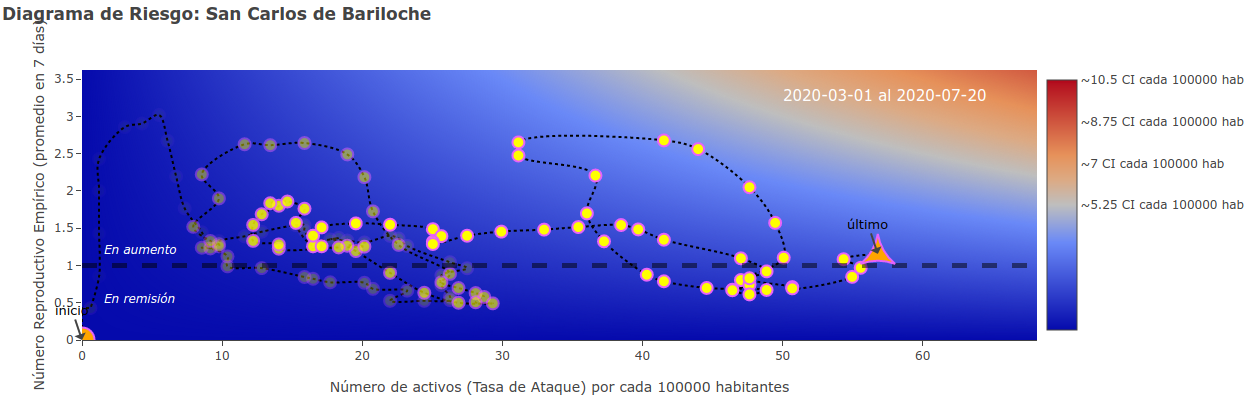
\includegraphics[width=14cm,clip=true]{bari.png}
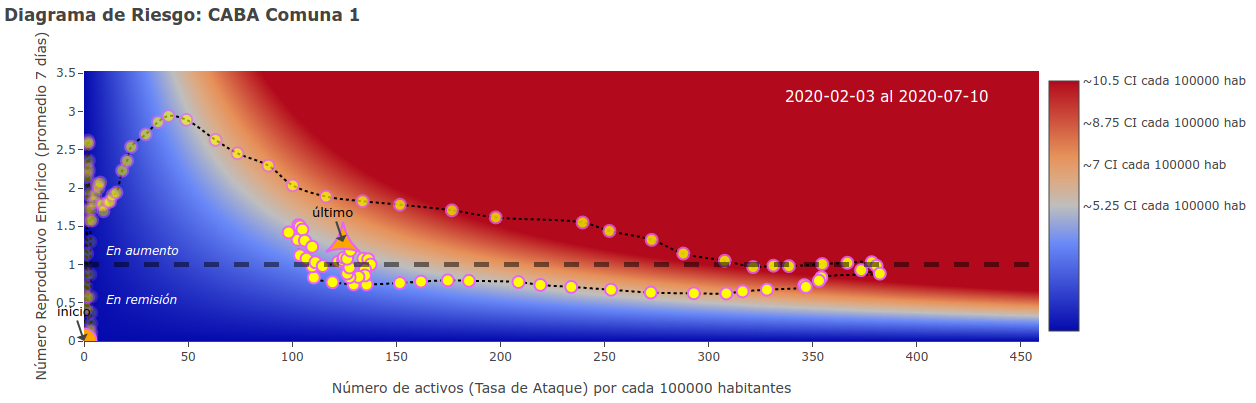
\includegraphics[width=14cm,clip=true]{cabacomuna1.png}
\end{center}
\caption{
Ejemplos de diagramas de riesgo, para ciudad de San Carlos de 
Bariloche (arriba) y para la Comuna 1 (Retiro), de la Ciudad Autonoma de Buenos 
Aires (abajo).
}
\label{fig:bari}
\end{figure}
En la figura \ref{fig:bari} se muestra un ejemplo, para la ciudad 
de San Carlos de Bariloche y para una de las comunas de la 
Ciudad Autonoma de Buenos Aires. Cada punto en los diagramas 
representa la situación un día dado, y el triángulo muestra 
el indicador calculado para el día más reciente que permiten los datos.
El fondo de color representa el grado de riesgo, y para cuantificarlo 
la barra de color de la derecha hace una correspondencia aproximada 
entre el color y el número de ciudados intensivos adicionales predicho.


Es interesante observar la evolución temporal en el diagrama de riesgo.
En la figura \ref{fig:bari} observamos que en Bariloche, la epidemia 
esta controlada por una secuencia de brotes. 
En un dado brote, el número de 
activos aumenta por un tiempo pero luego se contiene. El 
número reproductivo baja por debajo de $1$, y los activos 
empiezan a recuperarse haciendo que el número de activos
disminuya y el punto se desplace a la izquierda. Un nuevo 
brote aparece cuando nuevamente $R^7_t>1$. 
En la comuna 1 de CABA se observan muchos menos de 
estos brotes y una estructura mas suave, debido al tamaño 
de la población. 
En los últimos días disponibles para cada población 
puede observarse que mientras para Bariloche el número de cuidados 
intensivos adicionales es del orden de $2$, para la comuna 1 de CABA
es del orden de $5$ por cada 100000 habitates. Por supuesto, 
la gravedad de cada caso debe evaluarse de acuerdo a la 
capacidad sanitaria de cada población.


%Viendo como evoluciona este índice: mejorando
%(hacia abajo y a la izquierda), o empeorando (hacia arriba y a la derecha).
%En la Figura 1 puede verse el diagrama de riesgo para Bariloche. El fondo de color indica el
%valor del riesgo, donde el riesgo aumenta hacia los rojos y disminuye hacia los azules.
%El nivel de riesgo asociado a un valor dado de EPG está determinado por la capacidad del
%sistema sanitario, en este caso de Bariloche.
%Para el gráfico de riesgo de la Figura 1, consideramos que en Bariloche, cada cien mil
%habitantes, DTL=782 (según el registro histórico), C estimado como la suma de UTIs + UCIs
%libres en la última fecha, y que la fracción de internación de testeados positivos en UTIs +
%UCIs es del 3.5% aproximadamente, es decir f=0.035 (estimado a partir de estadísticas de
%Argentina).
%En el caso de Bariloche se observa una evolución cíclica en el tiempo del índice de riesgo.
%Los días de valores altos de EPG en Bariloche (Figura 1 arriba y a la derecha) coincidieron
%con los días de mayor número de casos (11 de Abril y 15 de Mayo), pero además con un
%alto número de casos activos en los días siguientes .
%Según este indicador de riesgo, la dinámica cíclica de casos en Bariloche hasta el momento
%parece evolucionar en forma de brotes que no se solapan temporalmente. Esto está
%directamente relacionado con las características de una ciudad relativamente chica, en la
%que los brotes ocurren localmente y separados espacialmente.
%Los brotes se suceden en forma cíclica, debido posiblemente a la implementación de
%medidas alternadas de cuarentena más estricta y más relajada.
%Las medidas de contención deberían apuntar a llevarnos a la zona del diagrama de riesgo
%de abajo a la izquierda, por debajo de la línea de rho7 igual a 1, donde se dan las condiciones
%para que no ocurran brotes.
%3Figura 1: En el eje y, la tasa reproductiva diaria promedio Rho7 ( rho7 ). En el eje x la incidencia acumulada en los
%últimos 14 días (o Tasa de ataque) . Los colores indican el grado de riesgo de aparición de nuevos brotes en los
%siguientes días (azul bajo riesgo, rojo alto riesgo). Cada punto corresponde a un día, aumentando la intensidad
%del color de punto a medida que el tiempo avanza. El punto inicial corresponde al 26 de febrero (esquina
%inferior izquierda), el último día está indicado con un triángulo naranja.
%Para el caso de la provincia de Río Negro (Figura 2) se observa que actualmente el valor de
%Rho7 se encuentra cercano a 1.5 y por lo tanto dentro del régimen exponencial. Al mismo
%tiempo se ve una tendencia al aumento de la tasa de ataque, debido al aumento del
%número de casos positivos en los últimos 14 días.
%Es importante destacar que en este caso se uso la misma escala de colores para el riesgo
%en la ciudad de Bariloche. Para adaptar esta escala de riesgo a la de la Provincia de Río
%Negro habria que conocer la suma de UTIs + UCIs libres en la última fecha. De manera que
%la escala de riesgo se modifica día a día según los recursos disponibles del sistema
%sanitario.
%4Figura 2: En el eje y, la tasa reproductiva diaria Rho7 ( rho7 ). En el eje x la incidencia acumulada en los últimos
%14 días (o Tasa de ataque) . Los colores indican el grado de riesgo de aparición de nuevos brotes en los
%La escala de riesgo de este gráfico fue
%calculada según límites de capacidad de tests y hospitalaria de Bariloche y debe ser
%adaptada al caso de Río Negro.
%siguientes días (azul bajo riesgo, rojo alto riesgo).
%Las medidas de contención deberían apuntar a bajar la tasa reproductiva idealmente por
%debajo de 1 y a disminuír el número de casos, de manera de alejarse de la zona roja y
%moverse hacia abajo a la izquierda en la zona azul.
\section*{Datos}
Todos los datos utilizados para todos los diagramas de riesgo 
son públicos y provistos por el Ministerio de Salud de la Nación.
La calidad de los indicadores depende fuertemente de la calidad de los datos.
\begin{figure}
\begin{center}
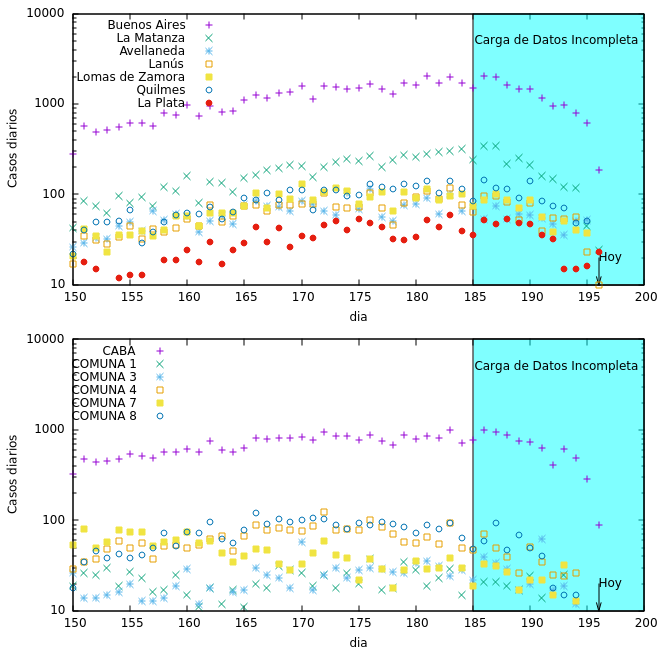
\includegraphics[width=14cm,clip=true]{datosdemorados2.png}
\end{center}
\caption{
Ejemplos de series temporales públicas 
obtenidas del Ministerio de Salud de la Nación. 
Se indica una anomalía, una disminución aparente pero artificial 
del número de casos positivos los últimos días, 
que es resultado de la carga lenta de los datos de 
algunas poblaciones. Estas demoras, que pueden llegar a ser de diez días, 
son sistemáticas y nos impiden hacer predicciones precisas así como obervar la 
dinámica más reciente. 
}
\label{fig:lento}
\end{figure}



Una de las dificultades más importantes para poder hacer predicciones epidemológicas es la carga lenta de los datos diarios. La figura \ref{fig:lento} muestra un ejemplo, extraído de fuentes oficiales del Ministerio de Salud de la Nación (\hyperref[https://sisa.msal.gov.ar/datos/descargas/covid-19/]{casos diarios}). En las poblaciones referidas se puede observar una caída sistemática del número de casos diarios los últimos días. Esta caída es \textit{artificial} y la misma estructura se repite día a día (es decir, solo se desplaza). Se debe a que las bases de datos no se actualizan rápidamente. En las poblaciones de la figura, se aprecia una demora de hasta 10 días.

Las fechas utilizadas corresponden a la \textit{fecha de inicio de síntomas}. Sin embargo otra de las dificultades encontradas con los datos es que la fecha de inicio de síntomas no está siempre reportada. En esos casos se ha utilizado la fecha de apertura, que ocurre varios días más tarde, a veces hasta 10 días mas tarde. Este problema no est\'a resuelto a\'un pero estaremos implementando pr\'oximamente una estimación estadística de la fecha de inicio de síntomas a partir de la de apertura.

Los datos poblacionales utilizados corresponden a la proyección del INDEC para 2020 y pueden encontrarse en \\

\verb|https://sitioanterior.indec.gob.ar/nivel4_default.asp?|\\
\verb|id_tema_1=2&id_tema_2=24&id_tema_3=119|

\section*{Advertencia}
La dinámica epídemica es muy compleja, y sería na\"{i}ve pensar que un solo indicador 
(como el tiempo de duplicación) o dos indicadores como los aquí discutidos nos permitan capturar todos los aspectos relevantes. En particular, la epidemia es compleja debido al alto grado heterogeneidad espacial y temporal dentro de cada población, y entran en juego 
innumerables variables sociales, económicas, geográficas, sanitarias, etc.
Es importante por lo tanto resaltar que es necesario trabajar con una variedad de indicadores seleccionados de manera que brinden, entre todos, una imagen completa del estado de situación. 


\section*{Consultas}
Para consultas relacionadas con los diagramas de riesgo, comunicarse con:\\

\noindent\fbox{%
    \parbox{8cm}{%
Dra. Karina Laneri \\
Grupo de Física Estadística e Interdisciplinaria \\
del Centro Atómico Bariloche\\ 
\texttt{karinalaneri@gmail.com}
    }%
}

\section*{Referencias}
Estos cálculos fueron realizados a partir del siguiente 
tutorial\\

\verb|https://biocomsc.upc.edu/en/shared/avaluacio_risc.pdf|\\

del grupo BIOCOMSC de la Universitat Politècnica de Catalunya. 
En particular, los diagramas de riesgo aquí descriptos fueron presentados
en reportes diarios para otros países (principalmente poblaciones europeas) 
por el grupo citado anteriormente, y pueden consultarse en el siguiente link:\\

\verb|https://biocomsc.upc.edu/en/covid-19|

\end{document}
